\section{Project Design and Methodology}\label{sec:chapter-4}

\subsection{Development approach}

The project documentation records an iterative development process organised around a 15-week journal. Early stages addressed problem definition, requirements, interface planning, and navigation. Subsequent work connected onboarding, check-ins, journals, authentication, persistent storage, content administration, and recommendations. Later changes introduced stronger privacy and comfort controls. The journal is a development record rather than independently verified time-sheet evidence. It supports an account of sequencing, but does not establish the exact effort spent on each activity.

Iterative delivery suits this artefact because changes in one component expose requirements in another. For example, device-only journal encryption changes both the journal API contract and the recommender's available inputs. Comfort preferences require corresponding metadata, backend mapping, fallback handling, and tests. Small vertical increments help expose these dependencies before the system is treated as complete. However, iteration can also leave older documentation inconsistent with newer source, so the report prioritises current routes and the journal-free evaluation over historical descriptions.

\begin{figure}[htbp]
\centering
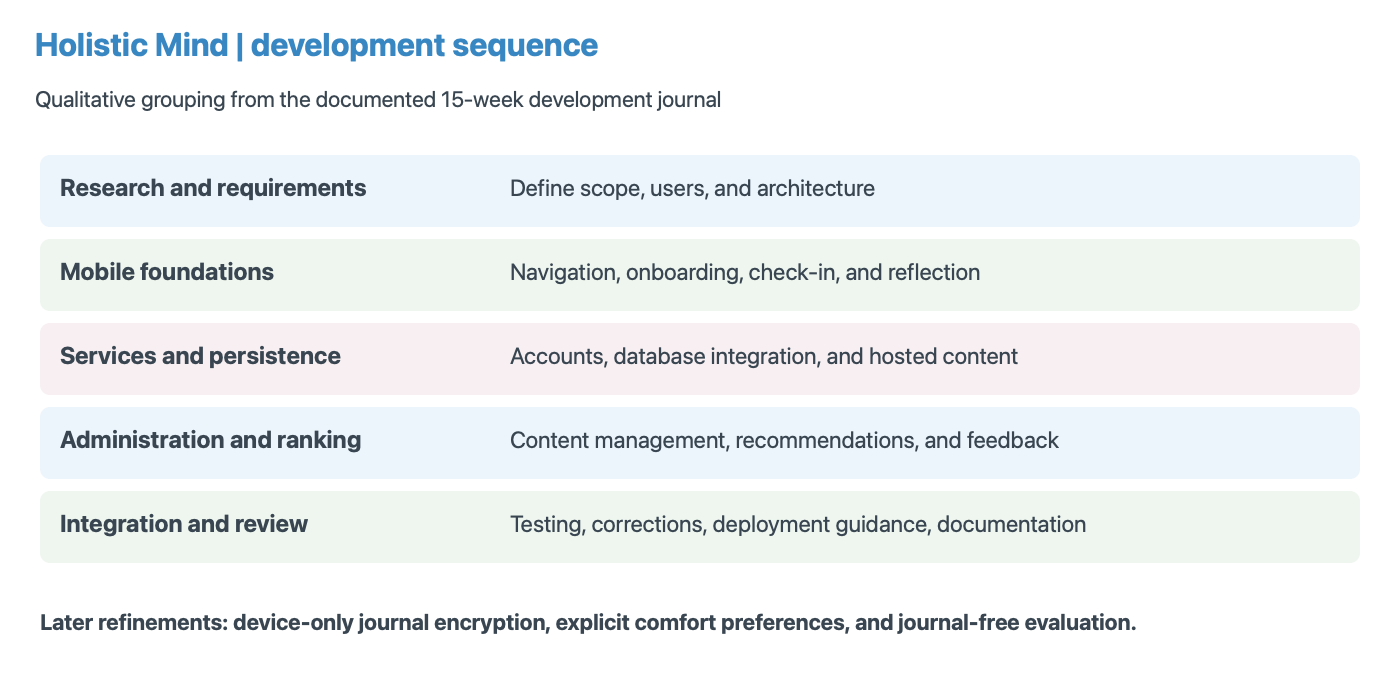
\includegraphics[width=\linewidth,height=0.62\textheight,keepaspectratio]{figures/timeline.png}
\caption[Development sequence]{Development phases summarised from the project's 15-week journal. Later privacy and evaluation refinements are shown separately; the graphic is a qualitative sequence, not measured effort.}
\label{fig:timeline}
\end{figure}
\FloatBarrier

\subsection{Technology selection}

Expo React Native and TypeScript provide a shared mobile implementation and typed integration between screens and services. Node.js with Express manages authenticated application operations, while PostgreSQL stores relational wellness and content records. A Python FastAPI service isolates numerical recommendation work from account and content APIs. ONNX inference keeps the pretrained embedding model within the recommendation service. The architecture adds operational complexity compared with a single process, but gives each component a clear responsibility.

Object storage holds larger media assets, avoiding their inclusion in ordinary database rows or every application bundle. A separate React administration interface allows structured content updates. These decisions are appropriate to the existing codebase and content requirements; they are not the result of a formal comparison of every available framework. Maintaining several runtimes, schema migrations, native builds, and storage policies remains a cost that must be considered alongside flexibility.

\subsection{Evidence and evaluation strategy}

The evaluation uses several evidence types because no single test answers all objectives. Offline ranking files compare recommendation approaches. Restriction tests exercise explicit exclusions and insufficient candidate pools. Journal cryptography and API tests address envelope validation, ownership, and migration. The device-and-backend record describes previous checks against a simulator and running development services. Source inspection establishes what is implemented, but it cannot demonstrate that a production deployment behaves identically.

The main ranking dataset contains 30 authored personas, each with relevance labels for all 14 benchmark exercises. Labels range from negative suitability to strongest relevance. The production suite removes synthetic journal inputs while retaining the original scenario labels. Ten repetitions per persona support timing measurement and random-baseline variation. They do not create 300 independent people. A separate eight-scenario suite examines declared comfort restrictions. The suites are reported separately because their purposes and input distributions differ.

\subsection{Ethical and methodological controls}

The report uses supplied dissertations as structural references without adopting their instructions, declarations, participant claims, or results. Existing project screenshots illustrate interfaces, while architectural figures explain source-observed behaviour. Reported benchmark values come from saved project artefacts. No new participant study is invented, and documented development passes are attributed to their original test record. This separation makes it possible to assess implementation without implying evidence that does not exist.

Privacy is considered throughout the architecture rather than added only to the discussion. Journal encryption reduces server access to reflective content, while structured check-ins and interaction data remain server-readable. The distinction should be explained to users. Synthetic scenarios reduce the need to expose real journals during development, but cannot replace independent expertise or diverse real-world experience. Any later user study should define consent, withdrawal, data minimisation, and a suitable research protocol before recruitment.

\subsection{Design Science Research framing}

\citet{hevner2004} describe design science as research through building and evaluating information-system artefacts. This provides the methodological foundation proposed in the April interim report. Holistic Mind instantiates that approach through an application, a recommendation mechanism, and a privacy architecture that respond to a defined problem. The research contribution is assessed through documented behaviour and evaluation, rather than the existence of code alone.

The project's problem phase identified fragmented daily support and the burden of choosing content. The construction phase developed the mobile interface and connected services. Evaluation then exposed practical issues: native dependencies missing from a build, secure-storage signing requirements, recommendation exclusions, and the impact of removing journal context. These findings prompted targeted refinements. The resulting learning is specific to the artefact: restrictions need a shared policy, privacy changes need new evaluation inputs, and native integration needs installed-build verification.

A limitation of the research process is that technical evaluation progressed further than evaluation with intended users. The artefact therefore has stronger evidence for data flow and restriction enforcement than for perceived usefulness. A mature DSR account should acknowledge that imbalance and specify what the next evaluation cycle must resolve. The report does so through a study protocol, independent content-review priorities, and a release-verification plan. This is a defensible partial research outcome rather than a claim that construction alone proves the design successful.

\subsection{User-centred design activities and boundaries}

The earlier reviews emphasised friendly onboarding and the risk of making sensitive questions clinical or overwhelming. That rationale is reflected in short options, supportive wording, and the ability to choose a support goal without describing traumatic experiences. Interface refinement also addressed spacing, card size, text wrapping, and navigation. These activities show attention to the user's interaction burden, although developer-led iteration is different from systematic observation of a representative user group.

The next user-centred cycle should test the user's understanding of the complete journey. A participant should be able to explain what a check-in contributes, distinguish a suggestion from an instruction, identify how to avoid a practice, and understand the recovery consequences of encrypted journaling. Observing these tasks would be more informative than asking only whether the screen looks attractive. It would also reveal whether privacy explanations create confusion or prevent a person from completing setup.

\subsection{Feasibility and resource constraints}

The April plan described a nine-month project, while the repository contains a fifteen-week development journal. These sources represent different planning views rather than interchangeable records of elapsed effort. The dissertation uses dated submissions to establish major milestones and the development journal to describe work phases. It does not infer an exact completion percentage from either. That avoids an apparent discrepancy being resolved through invented dates or effort estimates.

Technical feasibility rests on the existing integration of mature components: a shared mobile codebase, typed API modules, relational persistence, object storage, and a compact pretrained embedding model. Operational feasibility is more demanding because the project now contains multiple services and native dependencies. A stopped API can prevent sign-in despite correct Google configuration. A stale container can return an older ranking version despite updated source. These examples show why service readiness and version identification are practical requirements.

Content production is a separate resource constraint. Audio, video, written guidance, and curriculum structures require review and consistent metadata as well as upload tooling. The administration dashboard reduces release friction, but it does not remove that editorial workload. A staged content release is more feasible than assuming every proposed module can be produced and validated immediately. The original idea of optional later modules should remain a roadmap rather than a reason to delay validation of the core daily loop.

\subsection{Risk management and ethical feasibility}

The earlier reports identify recruitment difficulty, content delays, recommendation complexity, possible participant distress, and platform-release constraints. Their mitigation ideas remain useful, but Firebase billing risks are no longer an adequate description of the current system. Current operational risks include multi-service availability, public and private storage configuration, recovery-key loss, unsuitable metadata, and the compatibility of native builds with backend changes.

\begingroup
\small\setstretch{1.08}
\setlength{\tabcolsep}{4pt}
\setlength{\TableInnerWidth}{\dimexpr\linewidth-24pt\relax}
\begin{longtable}{@{}>{\raggedright\arraybackslash}p{0.250\TableInnerWidth} >{\raggedright\arraybackslash}p{0.290\TableInnerWidth} >{\raggedright\arraybackslash}p{0.180\TableInnerWidth} >{\raggedright\arraybackslash}p{0.280\TableInnerWidth}@{}}
\caption{Current project risk register. Ratings are qualitative planning judgments, not measured incident probabilities.}\label{tab:table-2}\\
\toprule
\textbf{Risk} & \textbf{Likelihood} & \textbf{Impact} & \textbf{Control or next action} \\
\midrule\endfirsthead
\multicolumn{4}{l}{\textit{Table \thetable\ continued}}\\
\toprule
\textbf{Risk} & \textbf{Likelihood} & \textbf{Impact} & \textbf{Control or next action} \\
\midrule\endhead
\midrule\multicolumn{4}{r}{\textit{Continued on next page}}\\\endfoot
\bottomrule\endlastfoot
Unreviewed exercise metadata & Medium & High & Independent review; version catalogue \\ \addlinespace[4pt]
Lost journal recovery material & Medium & High & Clear backup confirmation; recovery tests \\ \addlinespace[4pt]
Outdated app or container version & Medium & High & Version checks; coordinated release \\ \addlinespace[4pt]
Wrong storage access configuration & Medium & High & Separate public content from private data \\ \addlinespace[4pt]
Recruitment or ethics delay & Medium & Medium & Approve protocol before scheduling study \\ \addlinespace[4pt]
Media or content production delay & Medium & Medium & Publish reviewed core content in stages \\ \addlinespace[4pt]
Native signing or module mismatch & Medium & Medium & Test installed signed builds \\ \addlinespace[4pt]
Unclear recommendation explanation & Medium & Medium & Task-based usability assessment \\ \addlinespace[4pt]
\end{longtable}
\endgroup

Risk management should be proportionate to actual operations. Synthetic test accounts and fixtures permit technical verification without exposing real reflective histories. A future study with the intended audience requires its own consent process and support arrangements. The application should not ask participants to disclose a trauma story to qualify for a usability task. No claim of ethics approval, clinical review, or regulatory compliance is made merely because these controls appear in a plan.
